%\documentclass[iop]{emulateapj}
%\documentclass[12pt, preprint]{emulateapj}
\documentclass[12pt, onecolumn]{emulateapj}

\usepackage{amsmath}
%\usepackage{bibtex}
%\bibliographystyle{unsrtnat}

\newcommand{\myemail}{aimalz@nyu.edu}
\newcommand{\textul}{\underline}

%\slugcomment{}

\shorttitle{Probabilistic inference of the Hubble parameter}
\shortauthors{Malz and Peters, et al.}

\begin{document}

\title{Probabilistic inference of the Hubble parameter}

\author{Alex Malz\altaffilmark{1}}
\author{Tina Peters\altaffilmark{2}}
\author{Humna Awan}
\author{Anita Bahmanyar}
\author{Kara Ponder}
\author{Lluis Galbany}
\altaffiltext{1}{Center for Cosmology and Particle Physics, Department of Physics,
  New York University, 4 Washington Pl., room 424, New York, NY 10003, USA}
 \altaffiltext{2}{Dunlap\dots}
\email{aimalz@nyu.edu}

\begin{abstract}
The BEAMS framework enables the use of probabilistic supernova classifications to estimate the Hubble parameter quantifying the relationship between distance and redshift over cosmic time.  This work extends BEAMS to replace high-confidence spectroscopic redshifts with probabilistic photometric redshifts, enabling inference of the Hubble parameter as a function of two probabilistic variables.  By combining posterior probabilities of supernova type and posterior probability distributions over host galaxy redshift, we infer a posterior probability distribution over the redshift-dependent Hubble parameter.  This work also produces a code that can be used for other regression problems in astrophysics that involve catalogs of two probabilistic variables.
\end{abstract}

\keywords{}

\section{Introduction}
\label{sec:intro}

\citet{kunz_bayesian_2007, kelly_flexible_2008}

\section{Methods}
\label{sec:meth}

This covers a complete sample, i.e. a catalog of all $N$ supernovae $ns$ in the universe, ever.  We'll add in the selection function later.

Test reference Fig. \ref{fig:pgm}

\vspace{1in}
\begin{figure}
\begin{center}
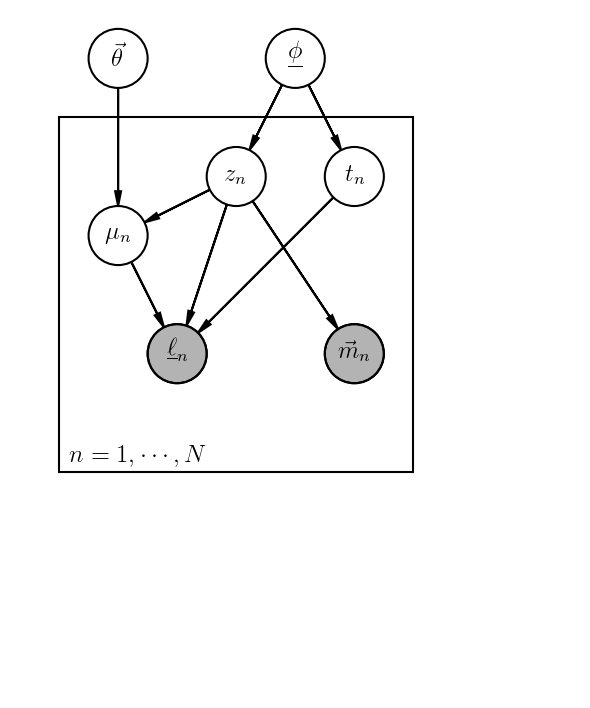
\includegraphics{Hubble-draft.png}
\caption{This directed acyclic graph corresponds to a probabilistic graphical model for our hierarchical inference of the Hubble parameter.  In this graph, all random variables are shown in circles, with observed variables shown in shaded circles.  The box indicates that there are $N$ copies of the relationships between boxed parameters, each independent of all others.  The hyperparameters we would like to infer are the cosmological parameters in $\vec{theta}$ and the supernova type-redshift distribution parameters comprising $\textul{\Phi}$.  Drawn from functions of these hyperparameters are the distance moduli $\{\mu_{n}\}_{N}$, redshifts $\{z_{n}\}_{N}$, and supernova types $\{T_{n}\}_{N}$.  Here, we observe host galaxy fluxes $\{\vec{f}_{n}\}_{N}$ and multi-band supernova lightcurves $\{\textul{\ell}_{n}\}_{N}$, shown in shaded circles.}
\label{fig:pgm}
\end{center}
\end{figure}
\vspace{1in}

The goal here is to constrain the posterior distribution of the hyperparameters of interest given the data, .

We first expand this in terms of Bayes' Rule.

\begin{align}
p(\vec{\theta}, \textul{\Phi} | \{\textul{\ell}_{n}\}_{N}, \{\vec{f}_{n}\}_{N}) &\propto p(\vec{\theta}, \textul{\Phi})\ p(\{\textul{\ell}_{n}\}_{N}, \{\vec{f}_{n}\}_{N} | \vec{\theta}, \textul{\Phi})
\end{align}

Next, we invoke the independence of the supernova parameters and observations; the $n^{th}$ system's parameters and data are assumed to be independent of the $(n+1)^{th}$ system's parameters and data.

\begin{align}
p(\{\textul{\ell}_{n}\}_{N}, \{\vec{f}_{n}\}_{N} | \vec{\theta}, \textul{\Phi}) &= \prod_{n}^{N}p(\textul{\ell}_{n}, \vec{f}_{n} | \vec{\theta}, \textul{\Phi})
\end{align}

Next, we use marginalization of the latent variables, because we do not wish to estimate their values directly.

\begin{align}
p(\textul{\ell}_{n}, \vec{f}_{n} | \vec{\theta}, \textul{\Phi}) &= \iiint p(\textul{\ell}_{n}, \vec{f}_{n} | \mu_{n}, z_{n}, T_{n})\ p(\mu_{n}, z_{n}, T_{n} | \vec{\theta}, \textul{\Phi})\ d\mu_{n}\ dz_{n}\ dT_{n}
\end{align}

We note that the equation calls for likelihoods $\{p(\textul{\ell}_{n}, \vec{f}_{n} | \mu_{n}, z_{n}, T_{n})\}_{N}$, but what we have are interim posteriors $\{p(\mu_{n}, z_{n}, T_{n} | \textul{\ell}_{n}, \vec{f}_{n}, \vec{\theta}^{*}, \textul{\Phi}^{*})\}_{N}$ for some interim priors $\vec{\theta}^{*}, \textul{\Phi}^{*}$.  The interim priors represent the beliefs about the hyperparameters $\vec{\theta}, \textul{\Phi}$ that go into our calculation of the posteriors from the data; whether explicitly chosen (as in methods relying on a template library) or implicitly derived (as in methods relying on a training data set), the interim priors are always present in the calculation of posterior distributions from data.  We will thus have to transform the math to be in terms of quantities we actually have.  We do this by multiplying the likelihood by an inspired factor of unity, in terms of the interim posteriors.

\begin{align}
p(\textul{\ell}_{n}, \vec{f}_{n} | \mu_{n}, z_{n}, T_{n}) &= p(\textul{\ell}_{n}, \vec{f}_{n} | \mu_{n}, z_{n}, T_{n})\ \frac{p(\mu_{n}, z_{n}, T_{n} | \textul{\ell}_{n}, \vec{f}_{n}, \vec{\theta}^{*}, \textul{\Phi}^{*})}{p(\mu_{n}, z_{n}, T_{n} | \textul{\ell}_{n}, \vec{f}_{n}, \vec{\theta}^{*}, \textul{\Phi}^{*})}
\end{align}

We will expand the denominator of that factor of unity according to Bayes' Rule.

\begin{align}
p(\mu_{n}, z_{n}, T_{n}|\textul{\ell}_{n}, \vec{f}_{n}, \vec{\theta}^{*}, \textul{\Phi}^{*}) &= \frac{p(\mu_{n}, z_{n}, T_{n} | \vec{\theta}^{*}, \textul{\Phi}^{*})\ p(\textul{\ell}_{n}, \vec{f}_{n} | \mu_{n}, z_{n}, T_{n}, \vec{\theta}^{*}, \textul{\Phi}^{*})}{p(\textul{\ell}_{n}, \vec{f}_{n} | \vec{\theta}^{*}, \textul{\Phi}^{*})}
\end{align}

By the independence of different hierarchical levels in the probabilistic graphical model, we may split up the most daunting term in the above expression.

\begin{align}
p(\textul{\ell}_{n}, \vec{f}_{n} | \mu_{n}, z_{n}, T_{n}, \vec{\theta}^{*}, \textul{\Phi}^{*}) &= p(\textul{\ell}_{n}, \vec{f}_{n} | \mu_{n}, z_{n}, T_{n})\ p(\textul{\ell}_{n}, \vec{f}_{n} | \vec{\theta}^{*}, \textul{\Phi}^{*})
\end{align}

Noting the presence of $p(\textul{\ell}_{n}, \vec{f}_{n} | \mu_{n}, z_{n}, T_{n})$ and $p(\textul{\ell}_{n}, \vec{f}_{n} | \vec{\theta}^{*}, \textul{\Phi}^{*})$ in both the numerator and denominator for $p(\textul{\ell}_{n}, \vec{f}_{n} | \mu_{n}, z_{n}, T_{n})$, we cancel the like terms to express the individual likelihoods in terms of known quantities.

\begin{align}
p(\textul{\ell}_{n}, \vec{f}_{n} | \mu_{n}, z_{n}, T_{n}) &= \frac{p(\mu_{n}, z_{n}, T_{n} | \textul{\ell}_{n}, \vec{f}_{n}, \vec{\theta}^{*}, \textul{\Phi}^{*})}{p(\mu_{n}, z_{n}, T_{n} | \vec{\theta}^{*}, \textul{\Phi}^{*})}
\end{align}

We are now ready to plug the individual likelihoods into the marginalization.

\begin{align}
p(\textul{\ell}_{n}, \vec{f}_{n} | \vec{\theta}, \textul{\Phi}) &= \iiint p(\mu_{n}, z_{n}, T_{n} | \textul{\ell}_{n}, \vec{f}_{n}, \vec{\theta}^{*}, \textul{\Phi}^{*})\ \frac{p(\mu_{n}, z_{n}, T_{n} | \vec{\theta}, \textul{\Phi})}{p(\mu_{n}, z_{n}, T_{n} | \vec{\theta}^{*}, \textul{\Phi}^{*})}\ d\mu_{n}\ dz_{n}\ dT_{n}
\end{align}

Now we can plug the marginalization back into the product.

\begin{align}
p(\{\textul{\ell}_{n}, \vec{f}_{n}\}_{N} | \vec{\theta}, \textul{\Phi}) &= \prod_{n}^{N}\ \iiint p(\mu_{n}, z_{n}, T_{n} | \textul{\ell}_{n}, \vec{f}_{n}, \vec{\theta}^{*}, \textul{\Phi}^{*})\ \frac{p(\mu_{n}, z_{n}, T_{n} | \vec{\theta}, \textul{\Phi})}{p(\mu_{n}, z_{n}, T_{n} | \vec{\theta}^{*}, \textul{\Phi}^{*})}\ d\mu_{n}\ dz_{n}\ dT_{n}
\end{align}

And finally, we can plug the product back into Bayes' Rule.

\begin{align}
p(\vec{\theta}, \textul{\Phi} | \{\textul{\ell}_{n}, \vec{f}_{n}\}_{N}) &\propto p(\vec{\theta}, \textul{\Phi})\ \prod_{n}^{N}\ \iiint p(\mu_{n}, z_{n}, T_{n} | \textul{\ell}_{n}, \vec{f}_{n}, \vec{\theta}^{*}, \textul{\Phi}^{*})\ \frac{p(\mu_{n}, z_{n}, T_{n} | \vec{\theta}, \textul{\Phi})}{p(\mu_{n}, z_{n}, T_{n} | \vec{\theta}^{*}, \textul{\Phi}^{*})}\ d\mu_{n}\ dz_{n}\ dT_{n}
\end{align}

This is the posterior we will attempt to sample!

\section{Data}
\label{sec:data}

In order to simulate a mock dataset of posterior distributions $\{p(\mu_{n}, z_{n}, T_{n} | \textul{\ell}_{n}, \vec{f}_{n}, \vec{\theta}^{*}, \textul{\Phi}^{*})\}_{N}$ over supernova type, redshift, and distance modulus, we will have to employ a forward model.

We will set true values of the hyperparameters $\vec{\theta}_{0}$ and $\textul{\Phi}_{0}$ that we would like to recover by performing hierarchical inference on our mock data.  We will first draw pairs of true parameters $(T_{n}^{0}, z_{n}^{0})$ from $\textul{\Phi}_{0}$.  Then we will calculate the true $\mu_{n}^{0}$ according to [insert distance modulus equation here] from $z_{n}^{0}$ and $\vec{\theta}_{0}$.

Next, we will construct likelihoods for each supernova.  Still not sure I'm thinking about this part correctly\dots

\begin{align}
T_{n}' &\sim D[\vec{r}(T_{n})]\\
z_{n}' &\sim \vec{\Phi}(T_{n})\\
\mu_{n}' &= \mu(z_{n}', \vec{\theta})
\end{align}

%\acknowledgments

%\appendix

\bibliography{references}

\end{document}